% generated by scripts/pkl_to_latex.py
% source PKL : tscan_v1_L8_Ne8_U5_mode-uniform_nmin2_solver-gcg_full_restarts10_iter300_kmax5_tol1em09_t0.05to2_N21-32c2aa6cb1ca.pkl
% scan type  : tscan
% state      : gs
% requires   : \usepackage{pgfplots} \pgfplotsset{compat=1.18}
% colours match the matplotlib PDF (tab10 cycle)
\definecolor{gmeC0}{HTML}{1F77B4}
\definecolor{gmeC1}{HTML}{FF7F0E}
\definecolor{gmeC2}{HTML}{2CA02C}
\definecolor{gmeC3}{HTML}{D62728}
\definecolor{gmeC4}{HTML}{9467BD}
\definecolor{gmeC5}{HTML}{8C564B}
\definecolor{gmeC6}{HTML}{E377C2}
\definecolor{gmeC7}{HTML}{17BECF}

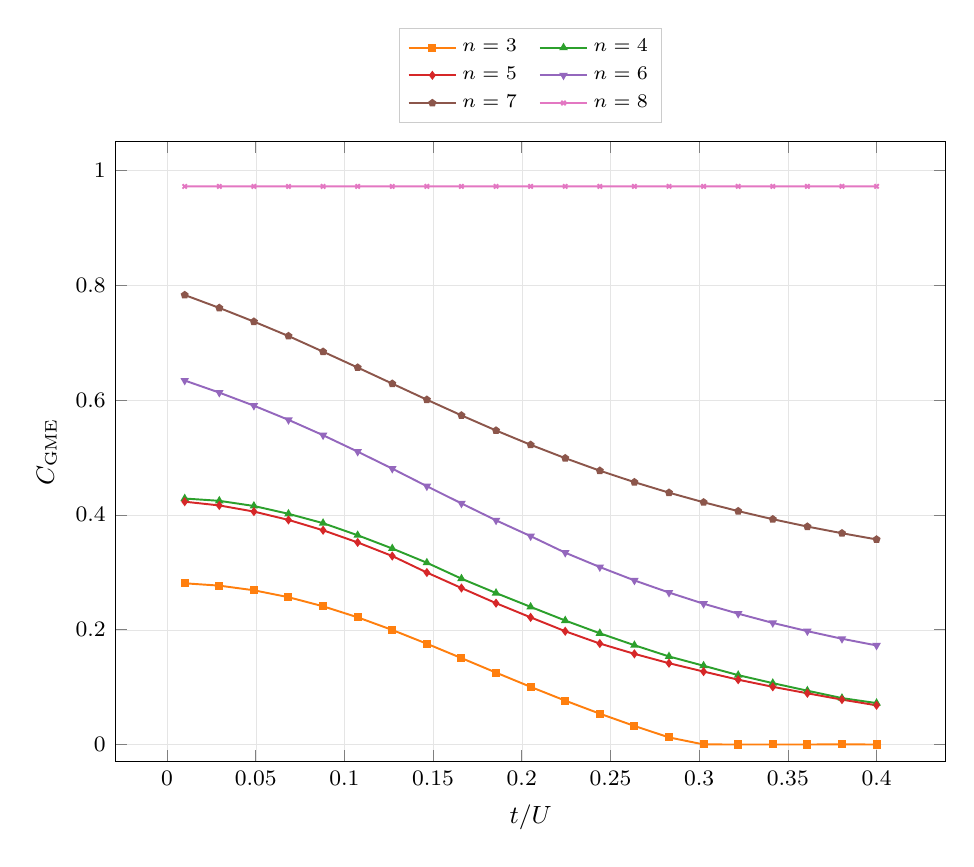
\begin{tikzpicture}
  \begin{axis}[
    width=\columnwidth,
    height=0.78\columnwidth,
    xlabel={$t/U$},
    ylabel={$C_{\mathrm{GME}}$},
    grid=both,
    grid style={line width=.1pt, draw=gray!20},
    tick label style={font=\footnotesize\rmfamily, /pgf/number format/fixed},
    label style={font=\small\rmfamily},
    scaled ticks=false,
    legend style={font=\scriptsize\rmfamily, draw=gray!40, at={(0.5,1.03)}, anchor=south, /tikz/every even column/.append style={column sep=6pt}},
    legend cell align={left},
    legend columns=2,
    ymin=-0.03,
    ymax=1.05,
  ]
    \addplot[color=gmeC1, mark=square*, mark size=1.1pt, line width=0.7pt] coordinates {
        (0.01,0.280758) (0.0295,0.276679) (0.049,0.268587) (0.0685,0.256542)
        (0.088,0.240717) (0.1075,0.22149) (0.127,0.199484) (0.1465,0.175517)
        (0.166,0.150483) (0.1855,0.125208) (0.205,0.100364) (0.2245,0.076428)
        (0.244,0.053698) (0.2635,0.032328) (0.283,0.012369) (0.3025,0.000128)
        (0.322,0.000038) (0.3415,0.000056) (0.361,0.000026) (0.3805,0.000221)
        (0.4,0.000009)
    };
    \addlegendentry{$n=3$}
    \addplot[color=gmeC2, mark=triangle*, mark size=1.1pt, line width=0.7pt] coordinates {
        (0.01,0.428367) (0.0295,0.424369) (0.049,0.415375) (0.0685,0.401725)
        (0.088,0.385471) (0.1075,0.364409) (0.127,0.341344) (0.1465,0.316551)
        (0.166,0.288826) (0.1855,0.263797) (0.205,0.239672) (0.2245,0.215943)
        (0.244,0.1937) (0.2635,0.172905) (0.283,0.153348) (0.3025,0.137181)
        (0.322,0.120833) (0.3415,0.106877) (0.361,0.093733) (0.3805,0.080817)
        (0.4,0.072144)
    };
    \addlegendentry{$n=4$}
    \addplot[color=gmeC3, mark=diamond*, mark size=1.1pt, line width=0.7pt] coordinates {
        (0.01,0.422845) (0.0295,0.416334) (0.049,0.405647) (0.0685,0.391136)
        (0.088,0.373102) (0.1075,0.351894) (0.127,0.328259) (0.1465,0.299493)
        (0.166,0.272518) (0.1855,0.246117) (0.205,0.221386) (0.2245,0.19726)
        (0.244,0.175801) (0.2635,0.157887) (0.283,0.141575) (0.3025,0.127042)
        (0.322,0.112886) (0.3415,0.100473) (0.361,0.089212) (0.3805,0.078167)
        (0.4,0.068264)
    };
    \addlegendentry{$n=5$}
    \addplot[color=gmeC4, mark=triangle*, mark size=1.1pt, mark options={rotate=180}, line width=0.7pt] coordinates {
        (0.01,0.633881) (0.0295,0.612825) (0.049,0.590064) (0.0685,0.565371)
        (0.088,0.538631) (0.1075,0.510015) (0.127,0.48042) (0.1465,0.44982)
        (0.166,0.41988) (0.1855,0.390387) (0.205,0.36284) (0.2245,0.334042)
        (0.244,0.30905) (0.2635,0.285777) (0.283,0.264624) (0.3025,0.245166)
        (0.322,0.227863) (0.3415,0.211755) (0.361,0.19742) (0.3805,0.18417)
        (0.4,0.172527)
    };
    \addlegendentry{$n=6$}
    \addplot[color=gmeC5, mark=pentagon*, mark size=1.1pt, line width=0.7pt] coordinates {
        (0.01,0.782789) (0.0295,0.760333) (0.049,0.736477) (0.0685,0.711336)
        (0.088,0.684064) (0.1075,0.656464) (0.127,0.628434) (0.1465,0.600476)
        (0.166,0.573185) (0.1855,0.546846) (0.205,0.521948) (0.2245,0.498639)
        (0.244,0.476863) (0.2635,0.456907) (0.283,0.438588) (0.3025,0.421819)
        (0.322,0.406487) (0.3415,0.392333) (0.361,0.379533) (0.3805,0.367926)
        (0.4,0.357147)
    };
    \addlegendentry{$n=7$}
    \addplot[color=gmeC6, mark=x, mark size=1.1pt, line width=0.7pt] coordinates {
        (0.01,0.971886) (0.0295,0.971886) (0.049,0.971887) (0.0685,0.971887)
        (0.088,0.971889) (0.1075,0.971891) (0.127,0.971894) (0.1465,0.971899)
        (0.166,0.971905) (0.1855,0.971912) (0.205,0.97192) (0.2245,0.97193)
        (0.244,0.97194) (0.2635,0.97195) (0.283,0.971961) (0.3025,0.971973)
        (0.322,0.971984) (0.3415,0.971996) (0.361,0.972008) (0.3805,0.97202)
        (0.4,0.972032)
    };
    \addlegendentry{$n=8$}
  \end{axis}
\end{tikzpicture}
